\documentclass[a4paper, 12pt]{article}

\usepackage[table,xcdraw]{xcolor}
\usepackage{enumerate}
\usepackage{graphicx}
\usepackage[T5]{fontenc}
\usepackage[utf8]{inputenc}
\usepackage[margin = 2cm]{geometry}
\usepackage{amsfonts, amsmath, amssymb}
\usepackage[none]{hyphenat}
\usepackage{fancyhdr}
\usepackage{float}
\usepackage{hyperref}
\usepackage{caption}
\usepackage[nottoc, notlot, notlof]{tocbibind}

% for code section
\usepackage{listings}

% for sub-figure
\usepackage{subcaption}
% \usepackage{rotating}
% \usepackage{tikz}

\captionsetup[table]{skip=5pt}
\pagestyle{fancy}
\fancyhead[L]{Trường Đại học Khoa học Tự nhiên - ĐHQG TP.HCM}
\fancyhead[R]{Nhóm 17}

\begin{document}
    \begin{titlepage}
        \begin{center}
            % \begin{table}[htbp]
            %     \begin{center}
            %     \begin{tabular}{cc}
            %         \includegraphics[scale = 1]{images/Picture1.png} & \begin{tabular}[c]{@{}l@{}}Đại học Quốc gia TP.HCM\\ Trường Đại học Khoa học Tự nhiên\end{tabular}
            %     \end{tabular}
            %     \end{center}
            % \end{table}

            \vspace*{1cm}
            \Large\textbf{Đại học Quốc gia TP. HCM\\Trường Đại học Khoa học Tự nhiên}\\

            \vfill
            \line(1,0){450}\\[4mm]
            \LARGE\textbf{\MakeUppercase{Báo cáo Lab 01\\ Mỗi quan hệ trong dữ liệu}}\\[3mm]
            \Large{Trực quan hoá dữ liệu (CSC10108)}\\[3mm]
            \Large{Nhóm 17}
            \line(1,0){430}\\
            \vfill

            \vfill
            TP Hồ Chí Minh, ngày 29/04/2021
        \end{center}
    \end{titlepage}

    \tableofcontents
    \thispagestyle{empty}
    \clearpage

    \section{Thông tin nhóm}
    \begin{table}[H]
        \begin{tabular}{|c|c|l|c|c|}
        \hline
        STT & MSSV     & \multicolumn{1}{c|}{Họ tên} & Email                         & SĐT        \\ \hline
        1   & 18120078 & Ngô Phù Hữu Đại Sơn         & 18120078@student.hcmus.edu.vn & 0919070940 \\ \hline
        2   & 18120201 & Nguyễn Bảo Long             & 18120201@student.hcmus.edu.vn & 0981850699 \\ \hline
        3   & 18120227 & Phạm Văn Minh Phương             & 18120227@student.hcmus.edu.vn & 0981850699 \\ \hline
        4   & 18120253 & Mai Ngọc Tú             & 18120253@student.hcmus.edu.vn & 0981850699 \\ \hline
        5   & 1712424 & Hàn Văn Gia Hiên            & 1712424@student.hcmus.edu.vn & 0911572108 \\ \hline
        \end{tabular}
        \caption{Bảng danh sách thành viên nhóm}
    \end{table}
    \clearpage

    \section{Phân tích hoàn thiện yêu cầu}

    \subsection{Tổng quan mức độ hoàn thành mỗi yêu cầu}

    \begin{table}[H]
        \begin{tabular}{|c|l|l|c|}
        \hline
        STT & \multicolumn{1}{c|}{Yêu cầu} & \multicolumn{1}{c|}{Công việc}                                                & Hoàn thành (\%) \\ \hline
        1 & Thu thập dữ liệu      & \begin{tabular}[c]{@{}l@{}}- Cài đặt chương trình thu thập dữ liệu\\ - Tiền xử lý dữ liệu\end{tabular}              & 100/100\\ \hline
        2 & Trực quan mối quan hệ & \begin{tabular}[c]{@{}l@{}}- Chọn trường dữ liệu cần trực quan\\ - Trực quan mối quan hệ, giải thích ý nghĩa, \\nhận xét biểu đồ\end{tabular}                          & 90/100 \\ \hline\end{tabular}
        \caption{Bảng phân tích đóng góp cá nhân}
    \end{table}

    \subsection{Mức độ hoàn thành của thành viên nhóm}

    \begin{table}[H]
        \begin{tabular}{|c|l|l|c|}
        \hline
        STT & \multicolumn{1}{c|}{Họ tên} & \multicolumn{1}{c|}{Công việc tham gia}                                                & Hoàn thành (\%) \\ \hline
        1 & Ngô Phù Hữu Đại Sơn      & \begin{tabular}[c]{@{}l@{}}- Thu thập dữ liệu\\- Hồi quy tuyến tính cho cá quan hệ\\ - Biểu diễn quan hệ 2 biến \& 4 biến\end{tabular}              & 100/100 \\ \hline
        2 & Nguyễn Bảo Long & \begin{tabular}[c]{@{}l@{}}- Biểu diễn quan hệ 3 biến \& 4 biến\\ - Giải thích lý do sử dụng biểu đồ đường\\ - Nhận xét dữ liệu 3 biến \& 4 biến\end{tabular}                          & 100/100 \\ \hline
        5 & Phạm Văn Minh Phương        & \begin{tabular}[c]{@{}l@{}}- Giải thích biểu đồ stacked bar chart\\ - Nhận xét dữ liệu stacked bar chart\end{tabular} & 100/100 \\ \hline
        5 & Mai Ngọc Tú       & \begin{tabular}[c]{@{}l@{}}- Giải thích biểu đồ scatter\\ - Nhận xét quan hệ dữ liệu 2 biến\end{tabular} & 100/100 \\ \hline
        5 & Hàn Văn Gia Hiên       & \begin{tabular}[c]{@{}l@{}}- Giải thích biểu đồ Worldmap\\ - Nhận xét dữ liệu biểu đồ Worldmap \end{tabular} & 100/100 \\ \hline
        \end{tabular}
        \caption{Bảng phân tích đóng góp cá nhân}
    \end{table}
    \clearpage

    \section{Thu thập dữ liệu}

    \subsection{Thu thập số liệu thống kê từng ngày}

    \begin{itemize}
        \item Nguồn dữ liệu: \url{https://www.worldometers.info/coronavirus/}
        \item Viết chương trình thu thập dữ liệu
        \begin{itemize}
            \item Ngôn ngữ: Python
            \item Framework: Scrapy - framework của python cho phép ta có thể cạo dữ liệu từ web site bằng các lớp đã được định nghĩa sẵn. Scrapy có 5 thành phần:
            \begin{enumerate}
                \item Spiders: Spiders là lớp đươc định nghĩa sẵn giúp ta có thể lấy dữ liệu liệu dự trên cấu trúc của website.
                Pipelines: Xử lý các thao tác tiền xử lý dữ liệu như: Làm sạch dữ liệu, xóa các phần tử trùng lặp.
                Middlewares: Xử lý các request gửi đến website và các response mà ta nhận lại được.
                Engine: Chịu trách nhiệm điều phối hoạt động của các thành phần khác.
                Sheduler: Chịu trách nhiệm duy trì thứ tự thực hiện của các công việc
            \end{enumerate}

            \item Các bước thực hiện
            \begin{enumerate}
                \item Cài đặt Scrapy
                \begin{verbatim}
    pip install Scrapy
                \end{verbatim}

                \item Tạo Scrapy project
                \begin{verbatim}
    scrapy startproject corona
                \end{verbatim}

                \item Tạo spider trong Scrapy
                \begin{verbatim}
    cd corona
    scrapy genspider covid www.worldometers.info/coronavirus
                \end{verbatim}

                \item Lấy dữ liệu từ xpath của trang HTML sau đó lưu vào Dataframe (Pandas). Cuối cùng, xuất dataframe ra file *.csv. Chi tiết cài đặt xem tại folder \textbf{crawler}.
                \item Lặp lại quá trình lấy dữ liệu theo ngày bằng đoạn script sau:
                \begin{verbatim}
    cd corona
    now=$(date +%d-%m)
    scrapy crawl covid -o ../../data/"$now".csv
    cd ..
                \end{verbatim}
            \end{enumerate}
        \end{itemize}
    \end{itemize}

    \subsection{Tiền xử lý}

    \begin{itemize}
        \item Dữ liệu dạng số sau khi lấy về có chứa dấu "," (ví dụ: 12,000) khiến cho máy tính "hiểu nhầm" là kiểu chuỗi.\\
        $\rightarrow$ Xoá dấu "," và các khoảng trắng dư thừa trong dữ liệu\\
        $\rightarrow$ Chuyển dữ liệu về dạng số
        $\rightarrow$ Điền giá trị 0 vào các ô dữ liệu trống

        \item Sau khi thực hiện xong các bước trên, xuất dữ liệu "sạch" ra một file *.csv mới.
        \item Chi tiết xem tại file \textbf{preprocess.py}
    \end{itemize}

    \subsection{Khám phá dữ liệu}

    \begin{itemize}
        \item Total Cases: Tổng số các ca nhiễm (gồm các ca nhiễm hiện có, đã tử vong, đã hồi phục).
        \item Total Deaths: Tổng số các ca nhiễm đã tử vong.
        \item Total Recovered: Tổng số các ca nhiễm đã hồi phục.
        \item Active Cases: Các ca nhiễm đang được điều trị.
        \item Total Tests: Tổng số lần xét nghiệm được thực hiện.
        \item Population: Dân số của một quốc gia.
    \end{itemize}

    \clearpage 

    \section{Trực quan hoá mối quan hệ giữa các trường dữ liệu}

    \subsection{Chọn trường dữ liệu}

    \begin{itemize}
        \item Với mỗi biến X, Y của tập dữ liệu, ta tính hệ số tương quan 
        \begin{equation}
            \rho(X, Y) = \frac{Cov(X, Y)}{\sqrt{Var(X)\times Var(Y)}} = \frac{Cov(X, Y)}{\sigma(X)\times \sigma(Y)}
        \end{equation}
        Với $Cov(X,Y) = E[XY] - E[X]E[Y]$ là hiệp phương sai của 2 biến X, Y.

        \item Từ đó, tính được ma trận hệ số tương quan giữa các cặp biến X, Y trong tập dữ liệu. Biểu diễn ma trận này bằng biểu đồ heatmap để xác định các trường dữ liệu trực quan.
        \begin{figure}[H]
            \begin{center}
                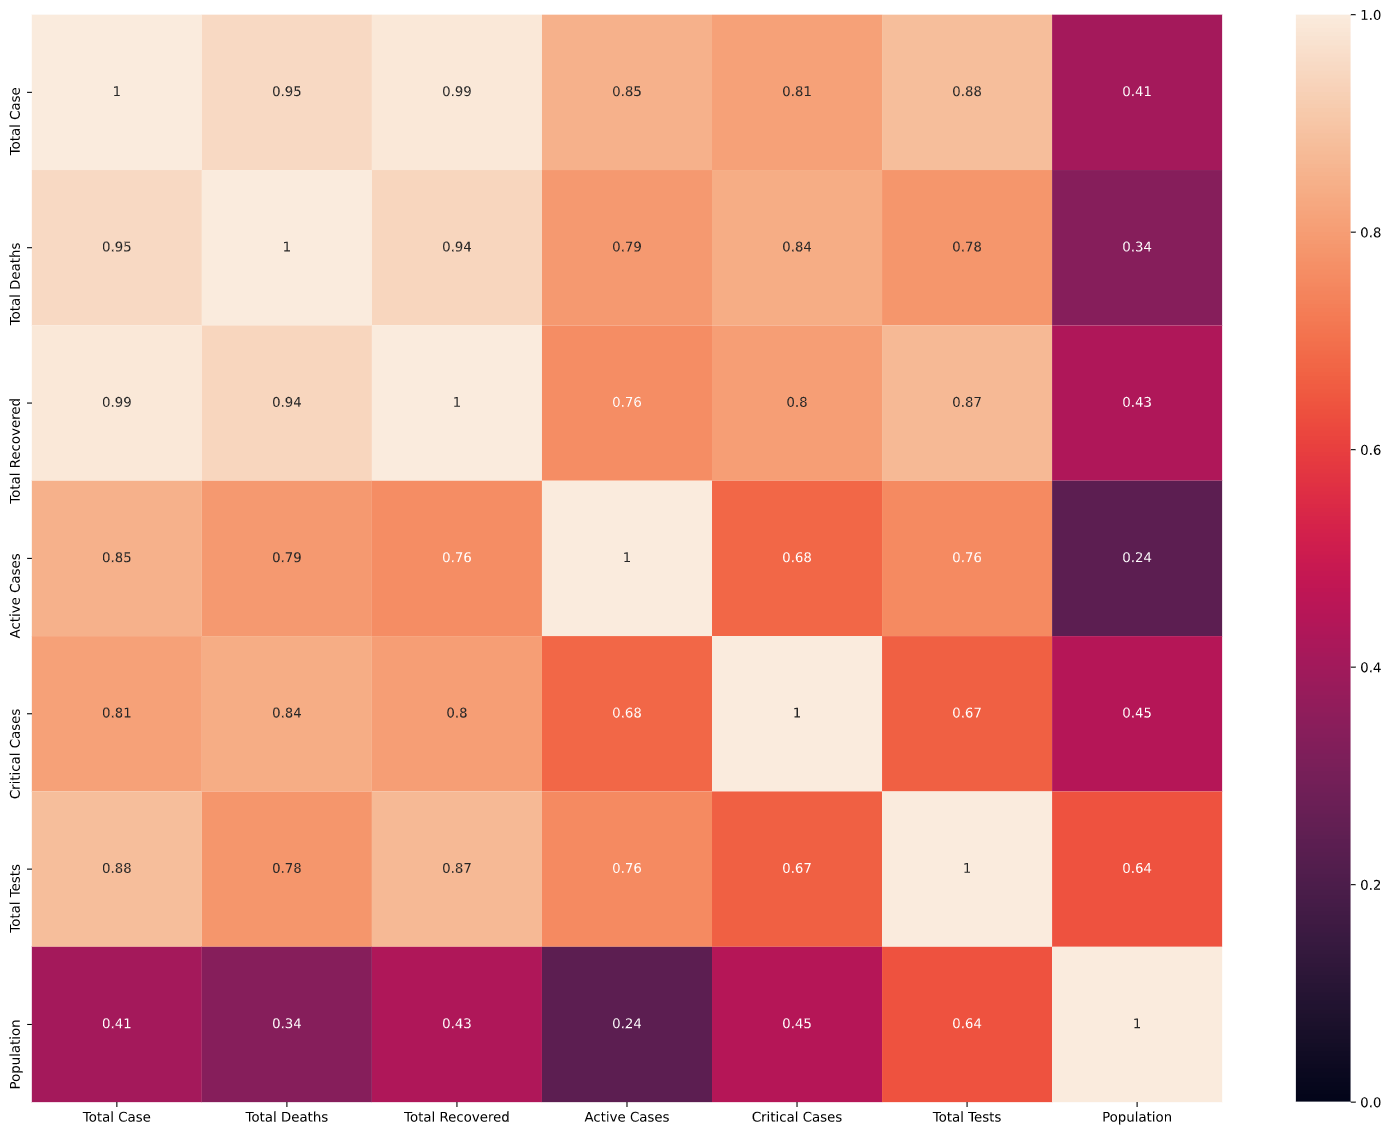
\includegraphics[scale = 0.3]{img/heatmap.png}
                \caption{Biểu đồ thể hiện hệ số tương quan giữa các trường dữ liệu}
            \end{center}
        \end{figure}

        \item Từ biểu đồ trên, chọn ra các cặp thuộc tính có hệ số tương quan lớn hơn 0.7, ta được bảng các cặp thuộc tính sau
        \begin{table}[H]
            \begin{center}
                \begin{tabular}{|c|c|c|c|}
                \hline
                \textbf{STT} & \textbf{Var1} & \textbf{Var2} & \textbf{Hệ số tương quan} \\ \hline
                1    &  Total Deaths     &  Total Cases    & 0.95                 \\ \hline
                2    &  Total Recovered  & Total Cases     & 0.99                 \\ \hline
                3    &  Total Recovered  & Total Deaths    & 0.94                 \\ \hline
                4    &  Active Cases     & Total Cases     & 0.85                 \\ \hline
                5    &  Active Cases     & Total Deaths    & 0.79                 \\ \hline
                6    &  Active Cases     & Total Recovered & 0.76                 \\ \hline
                7    &  Critical Cases   & Total Cases     & 0.81                 \\ \hline
                8    &  Critical Cases   & Total Deaths    & 0.84                 \\ \hline
                9    &  Critical Cases   & Total Recovered & 0.8                 \\ \hline
                10   &  Total Test       & Total Cases     & 0.88                 \\ \hline
                11   &  Total Test       & Total Deaths    & 0.78                 \\ \hline
                12   &  Total Test       & Total Recovered & 0.87                 \\ \hline
                13   &  Total Test       & Active Cases    & 0.76                 \\ \hline
                \end{tabular}
                \caption{Bảng các thuộc tính có hệ số tương quan trên 0.7}
            \end{center}
        \end{table}

        \item Từ bảng trên, ta thấy có 6 thuộc tính có mức độ tương quan với nhau cao là \textbf{Total Case, Total Deaths, Total Recovered, Active Cases, Critical Cases, Total Tests}. Do đó, ta tập trung vào tìm hiểu mối quan hệ giữa các thuộc tính này.
    \end{itemize}

    \subsection{Biểu diễn quan hệ giữa 2 trường dữ liệu}

    \begin{itemize}
        \item Với mỗi 2 trường dữ liệu X, Y trong danh sách các trường dữ liệu xuất hiện trong Table 4, trực quan các điểm dữ liệu thuộc 2 trường đó bằng biểu đồ scatter.
        \item Tiếp đó, tìm một quy luật xấp xỉ phù hợp nhất với dữ liệu quan sát bằng một đường thẳng $\bar{y} = w_0 + xw_1$ với $w_0, w_1$ được tính theo công thức sau
        \begin{equation}
            \left\{\begin{matrix}
                w_1 = \frac{\overline{XY} - \overline{X}.\overline{Y}}{\overline{X^2}-\overline{X}^2}\\w_0 = \overline{Y} - w_1\overline{X}
            \end{matrix}\right.
        \end{equation}

        \item Lý do sử dụng biểu đồ scatter kết hợp biểu diễn quy luật bằng một đường tuyến tính: Sử dụng biểu đồ scatter để trực quan giúp người đọc dễ dàng nhận ra một sự xấp xỉ tuyến tính (nếu có) tồn tại giữa 2 biến dữ liệu. Cộng thêm việc biểu diễn quy luật bằng một đường tuyến tính, người đọc có thể thấy rõ được "chất lượng" của đường tuyến tính này trong việc giải thích mối quan hệ giữa 2 trường dữ liệu.

        \item Kết quả thu được $C_6^2 = 15$  biểu đồ như sau
        \begin{figure}[H]
            \begin{center}
                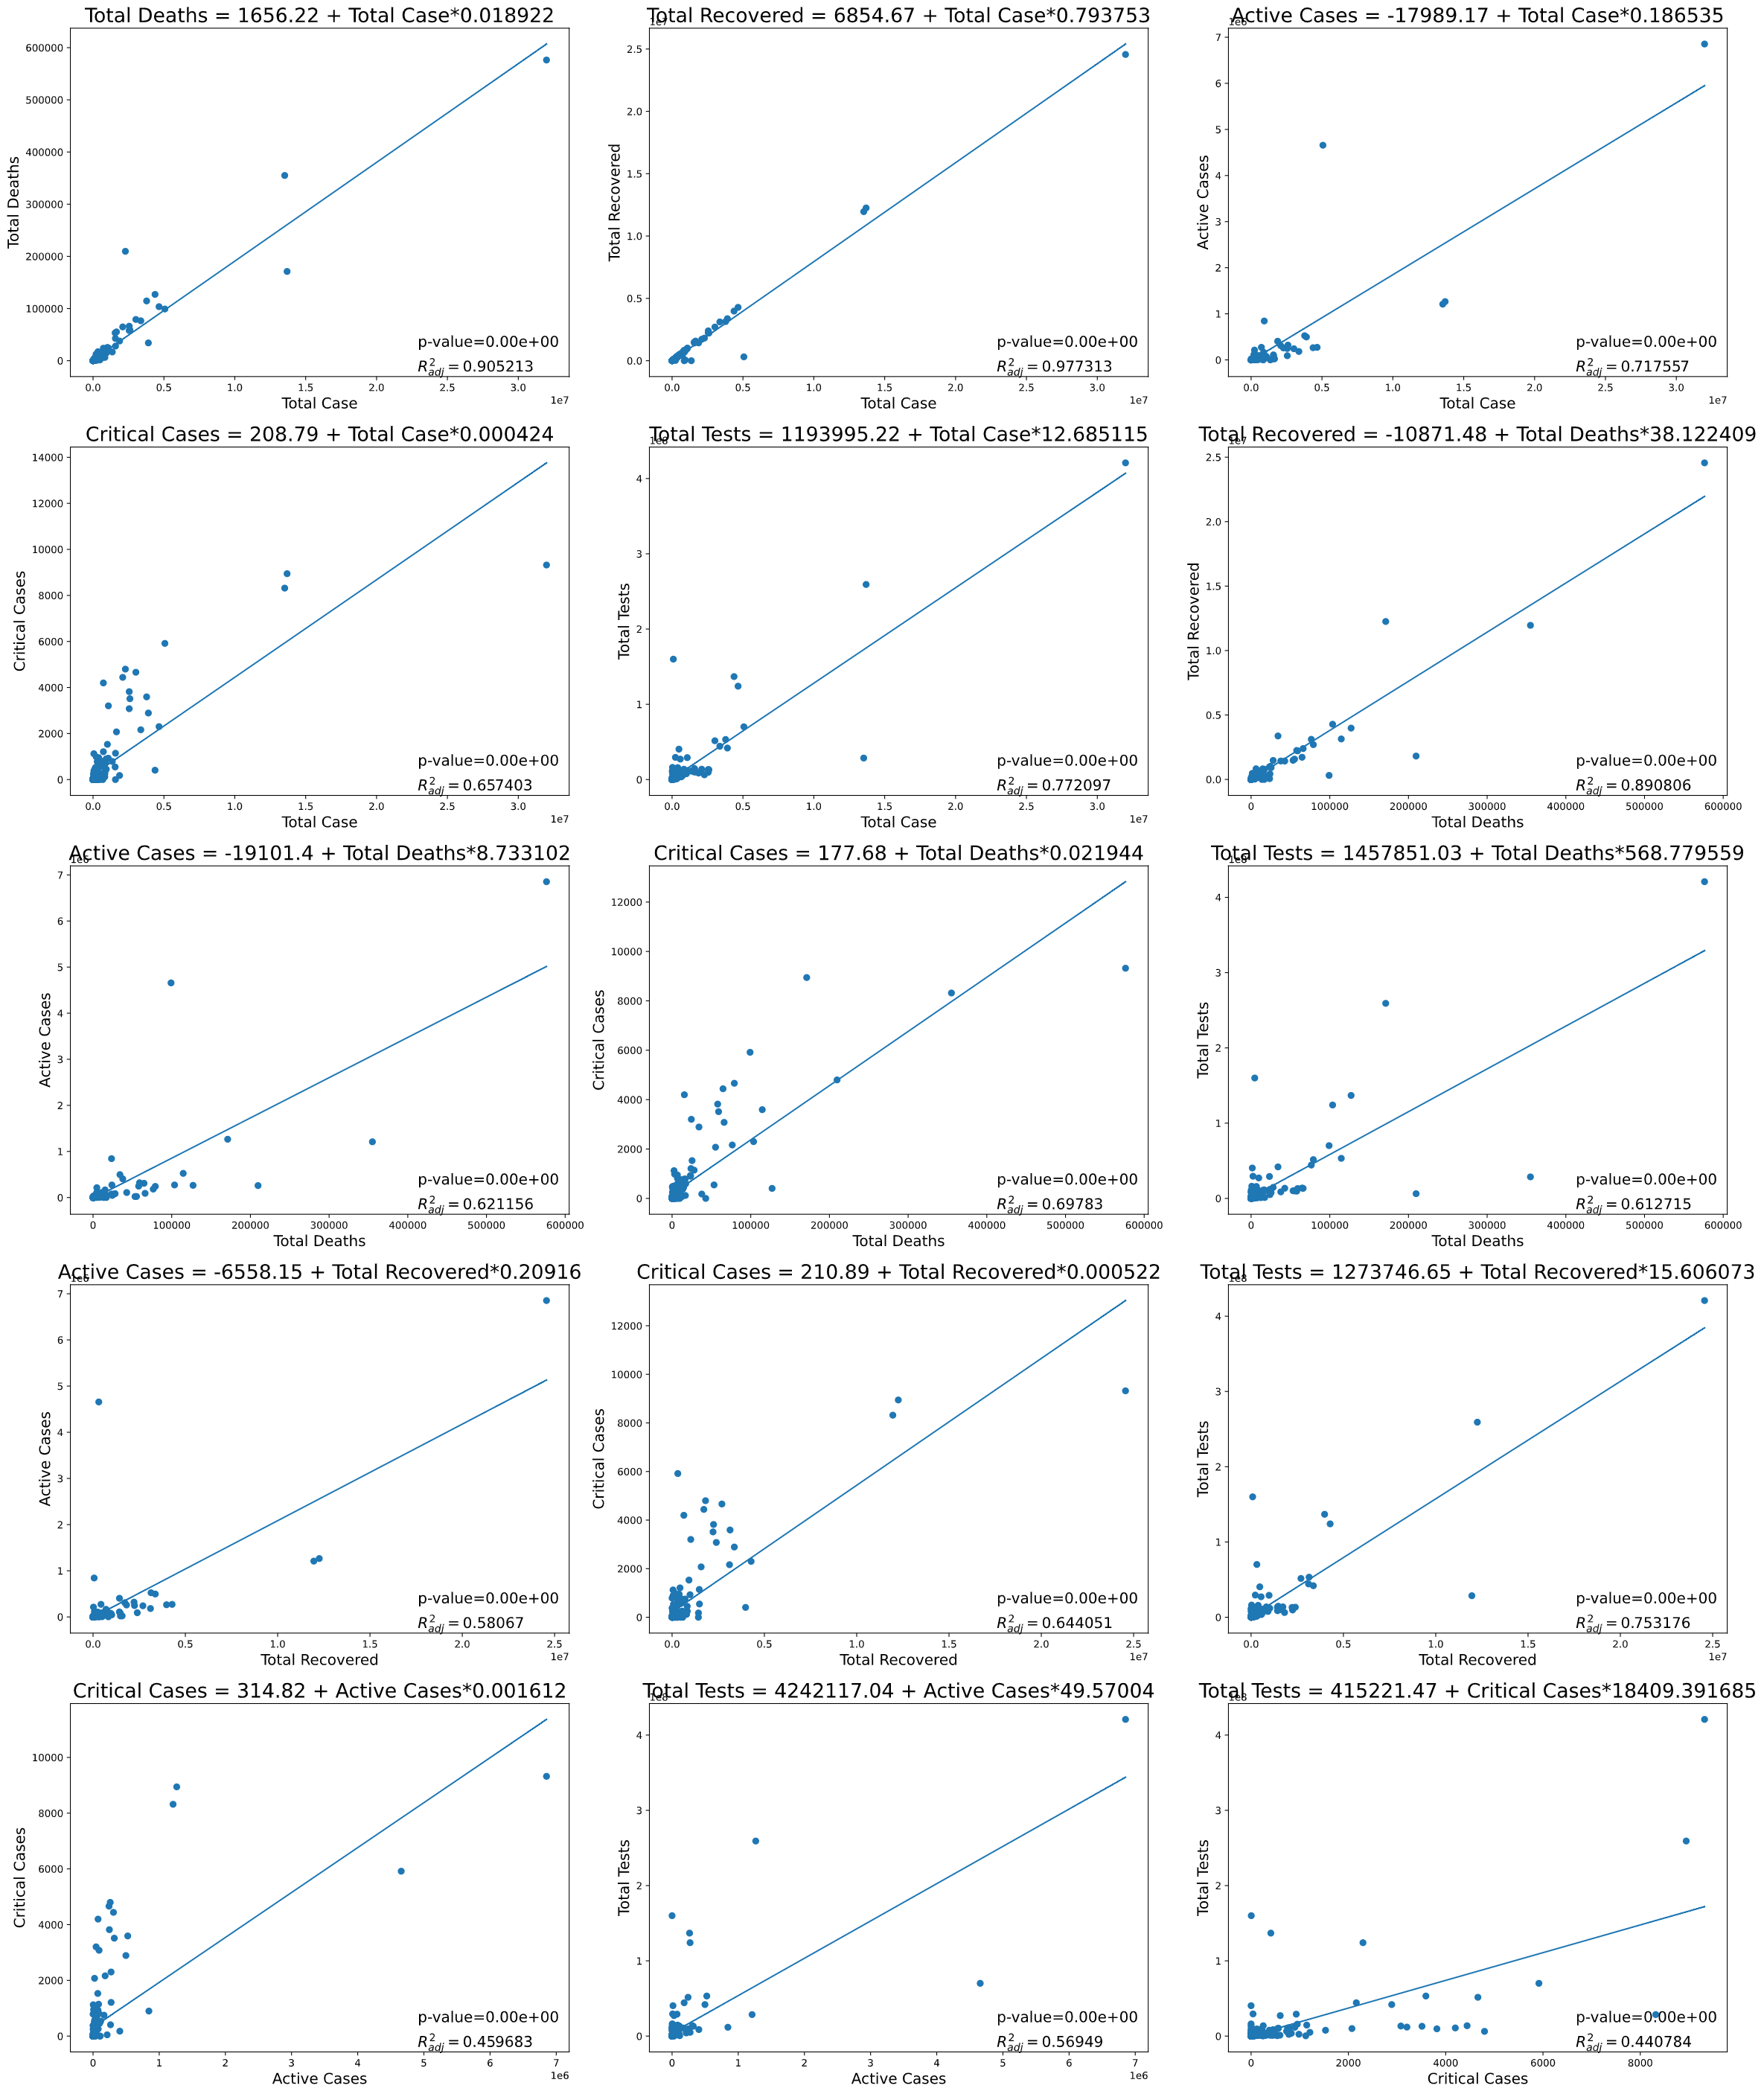
\includegraphics[scale=0.2]{img/scatter.png}
                \caption{Biểu đồ thể hiện mỗi quan hệ giữa 2 biến dữ liệu}
            \end{center}
        \end{figure}

        \item Nhận xét dữ liệu
        \begin{itemize}
            \item Với 5 cặp biến (Độc lập - Phụ thuộc): \textbf{(Total Case, Total Deaths), (Total Case, Total Recovered), (Total Case, Total Tests), (Total Deaths, Total Recovered), (Total Recovered, Total Tests)}, ta có các kết luận sau
            \begin{itemize}
                \item Chỉ số p-value của các cặp biến này rất nhỏ (trong khoảng [$10^{-180}, 10^{-68}$]). Do đó, các biến độc lập nêu trên có ý nghĩa về mặt thống kê.
                \item Mô hình phù hợp tốt với dữ liệu quan sát về mặt thống kê (p-value trong khoảng [$10^{-180}, 10^{-68}$]).
                \item Hệ số xác định hiệu chỉnh $R_{adj}^2$ của mỗi bộ dữ liệu đều nằm trong khoảng $[75\%, 98\%]$. Do đó, các biến độc lập giải thích được từ 75\% đến 98\% sự thay đổi của các biến phụ thuộc.
                \item Cụ thể phương trình hồi của các cặp biến được ghi trên biểu đồ.
            \end{itemize}

            \item Với các cặp biến còn lại, chỉ số $R_{adj}^2 < 75\%$. Do đó, việc giải thích sự thay đổi của biến phụ thuộc dựa trên biến độc lập là không đủ tin cậy.
        \end{itemize}
    \end{itemize}

    \subsection{Biểu diễn quan hệ giữa 3 trường dữ liệu}

    \begin{itemize}
        \item Với mỗi 3 trường dữ liệu X, Y, Z trong danh sách các trường dữ liệu xuất hiện trong Table 4, sử dụng kỹ thuật hồi quy tuyến tính để xác định một mặt phẳng xấp xỉ các điểm dữ liệu:
        \begin{equation}
            w = (X^T X)^{-1}X^Ty \text{, với X là ma trận các biến độc lập, y là biến phụ thuộc}
        \end{equation}
        \item Sau đó tính hệ số xác định hiệu chỉnh $R_{adj}^2$, ta xác định được các bộ 3 biến có $R_{adj}^2 > 70\%$ như sau
        \begin{table}[H]
            \centering
            \begin{tabular}{|c|c|c|c|c|} 
            \hline
            \textbf{ STT } & \textbf{ Var1 (độc lập) } & \textbf{ Var2 (độc lập) } & \textbf{ Var3 (phụ thuộc) } & \textbf{$R_{adj}^2$}  \\ \hline
            1              & Total Case                & Total Deaths              & Total Recovered             & 0.97                \\ \hline
            2              & Total Case                & Total Deaths              & Active Cases                & 0.71                \\ \hline
            3              & Total Case                & Total Deaths              & Total Tests                 & 0.80                \\ \hline
            4              & Total Case                & Total Recovered           & Active Cases                & 0.96                \\ \hline
            5              & Total Case                & Total Recovered           & Total Tests                 & 0.77                \\ \hline
            6              & Total Case                & Active Cases              & Total Tests                 & 0.77                \\ \hline
            7              & Total Case                & Critical Cases            & Total Tests                 & 0.77                \\ \hline
            8              & Total Deaths              & Total Recovered           & Total Tests                 & 0.76                \\ \hline
            8              & Total Recovered           & Active Cases              & Total Tests                 & 0.77                \\ \hline
            10             & Total Recovered           & Critical Cases            & Total Tests                 & 0.75                \\ \hline
            \end{tabular}
            \caption{Bảng các bộ 3 thuộc tính có mối tương quan trên 0.7}
        \end{table}

        \item Sử dụng biểu đồ đường để biểu diễn mối quan hệ giữa 3 biến dữ liệu như sau: Mỗi thuộc tính có một đường biểu diễn riêng. Giá trị này ứng với giá trị trên trục tung. Trục hoành là tên các quốc gia tương ứng.
        \item Lý do sử dụng biểu đồ đường
        \begin{itemize}
            \item Trước hết, chúng ta cần xác định mối quan hệ giữa 3 trường dữ liệu (bao gồm 2 trường độc lập và 1 trường phụ thuộc). Bằng kỹ thuật hồi quy tuyến tính (áp dụng phương trình (3)), giả sử ta tìm ra được hàm số sau:
            $$Total Recovered = f(Total Cases, Total Deaths) = 4556 + 0.8(Total Cases) + 1.4(Total Deaths)$$
            \item Lấy đạo hàm riêng của Total Recovered theo các biến độc lập, ta được
            \begin{itemize}
                \item $\frac{\partial{\text{ Total Recovered}}}{\partial{\text{ Total Cases}}} = 0.8 > 0$: Total Cases và Total Recovered biến thiên đồng biến. Nghĩa là khi Total Cases tăng thì Total Recovered cũng tăng theo (xét trong trường hợp Total Deaths là hằng số hoặc có biến động nhưng biến động này rất nhỏ so với các biến còn lại).
                \item $\frac{\partial{\text{ Total Recovered}}}{\partial{\text{ Total Deaths}}} = 1.4 > 0$: Total Deaths và Total Recovered biến thiên đồng biến. Nghĩa là khi Total Deaths tăng thì Total Recovered cũng tăng theo (xét trong trường hợp Total Cases là hằng số hoặc có biến động nhưng biến động này rất nhỏ so với các biến còn lại).
                \item Ngoài ra, $(\frac{\partial{\text{ Total Recovered}}}{\partial{\text{ Total Deaths}}} = 1.4) > (\frac{\partial{\text{ Total Recovered}}}{\partial{\text{ Total Cases}}} = 0.8)$: Total Recovered phụ thuộc vào Total Deaths nhiều hơn Total Cases.
            \end{itemize}

            \item Đối chiếu vào biểu đồ: Quan sát các tổng thể biểu đồ, ta thấy
            \begin{itemize}
                \item Total Deaths biến động rất nhẹ so với 2 biến còn lại. Do đó, sự thay đổi của biến này không ảnh hưởng nhiều đến Total Recovered.
                \item Total Cases biến động rất mạnh, và khi nó giảm/tăng thì Total Recovered (biến phụ thuộc) cũng giảm/tăng theo.
                \item Vậy ta đã biểu diễn được quan hệ biến thiên đồng biến giữa các biến Total Cases và Total Deaths với biến Total Recovered
            \end{itemize}
            \begin{figure}[H]
                \begin{center}
                    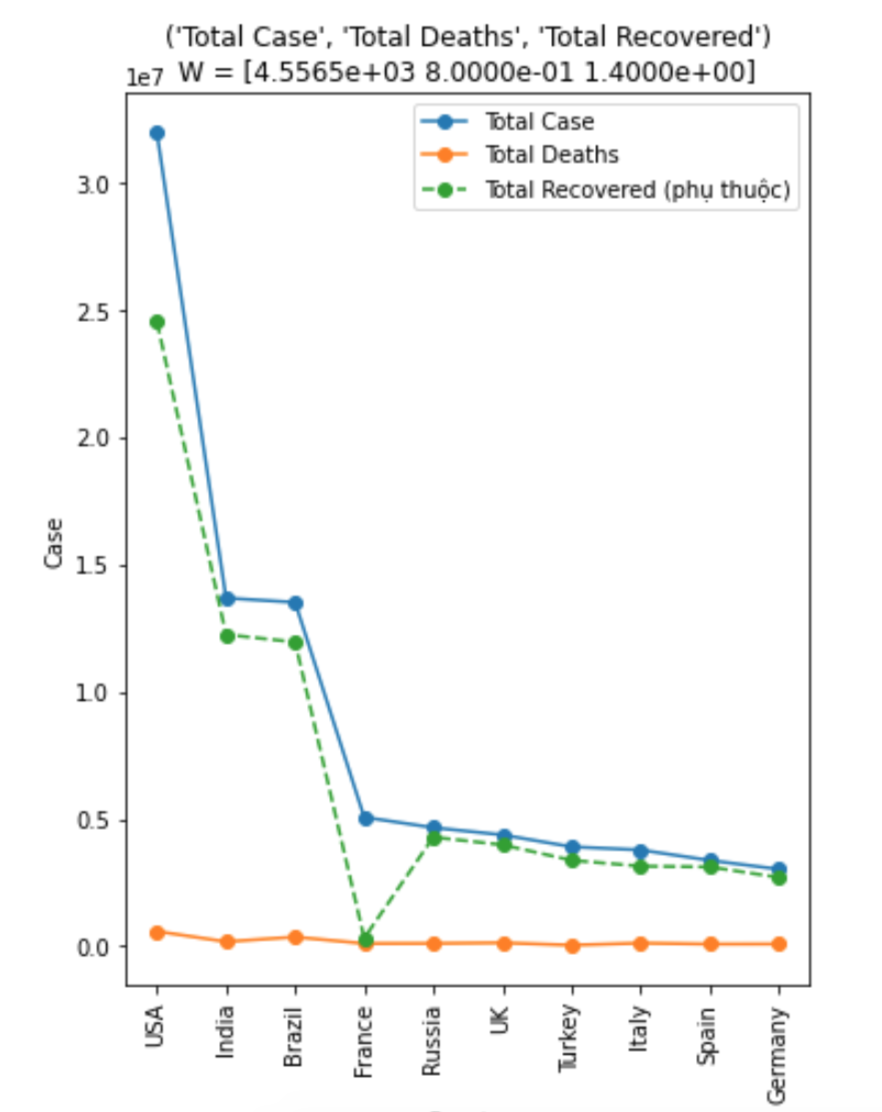
\includegraphics[scale=0.7]{img/lineChart.png}
                    \caption{Biểu đồ biểu diễn sự mối quan hệ của Total Cases, Total Deaths và Total Recovered}
                \end{center}
            \end{figure}

            \item Tóm lại, việc sử dụng biểu đồ đường để thể hiện mối quan hệ tuyến tính giữa các biến dữ liệu được nhóm cho là hợp lý vì đã biểu diễn được sự biến thiên phụ thuộc giữa các biến phụ thuộc và biến độc lập.
        \end{itemize}

        \item Trực quan các bộ 3 biến
        \begin{figure}[H]
            \begin{center}
                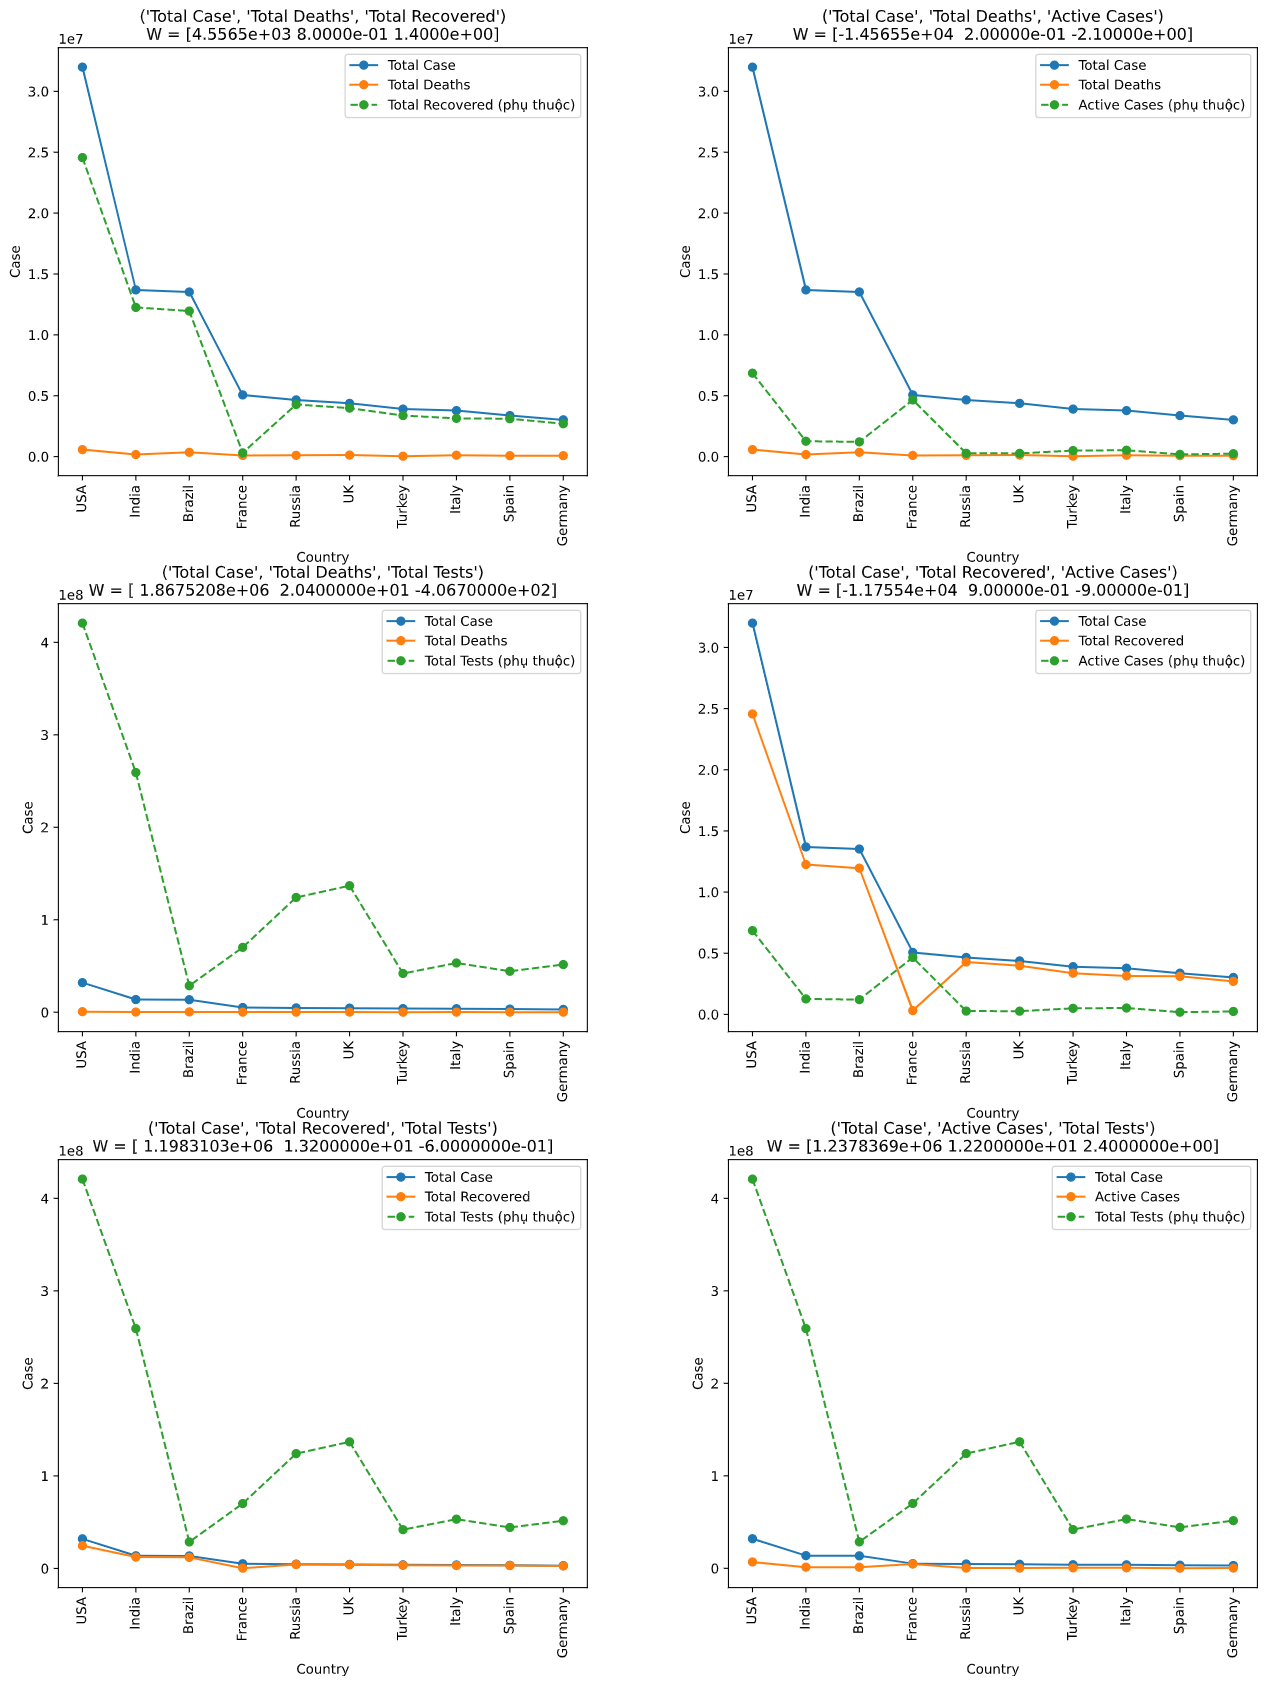
\includegraphics[scale=0.39]{img/relationship3Vars.png}
            \end{center}
        \end{figure}
        \begin{figure}[H]
            \begin{center}
                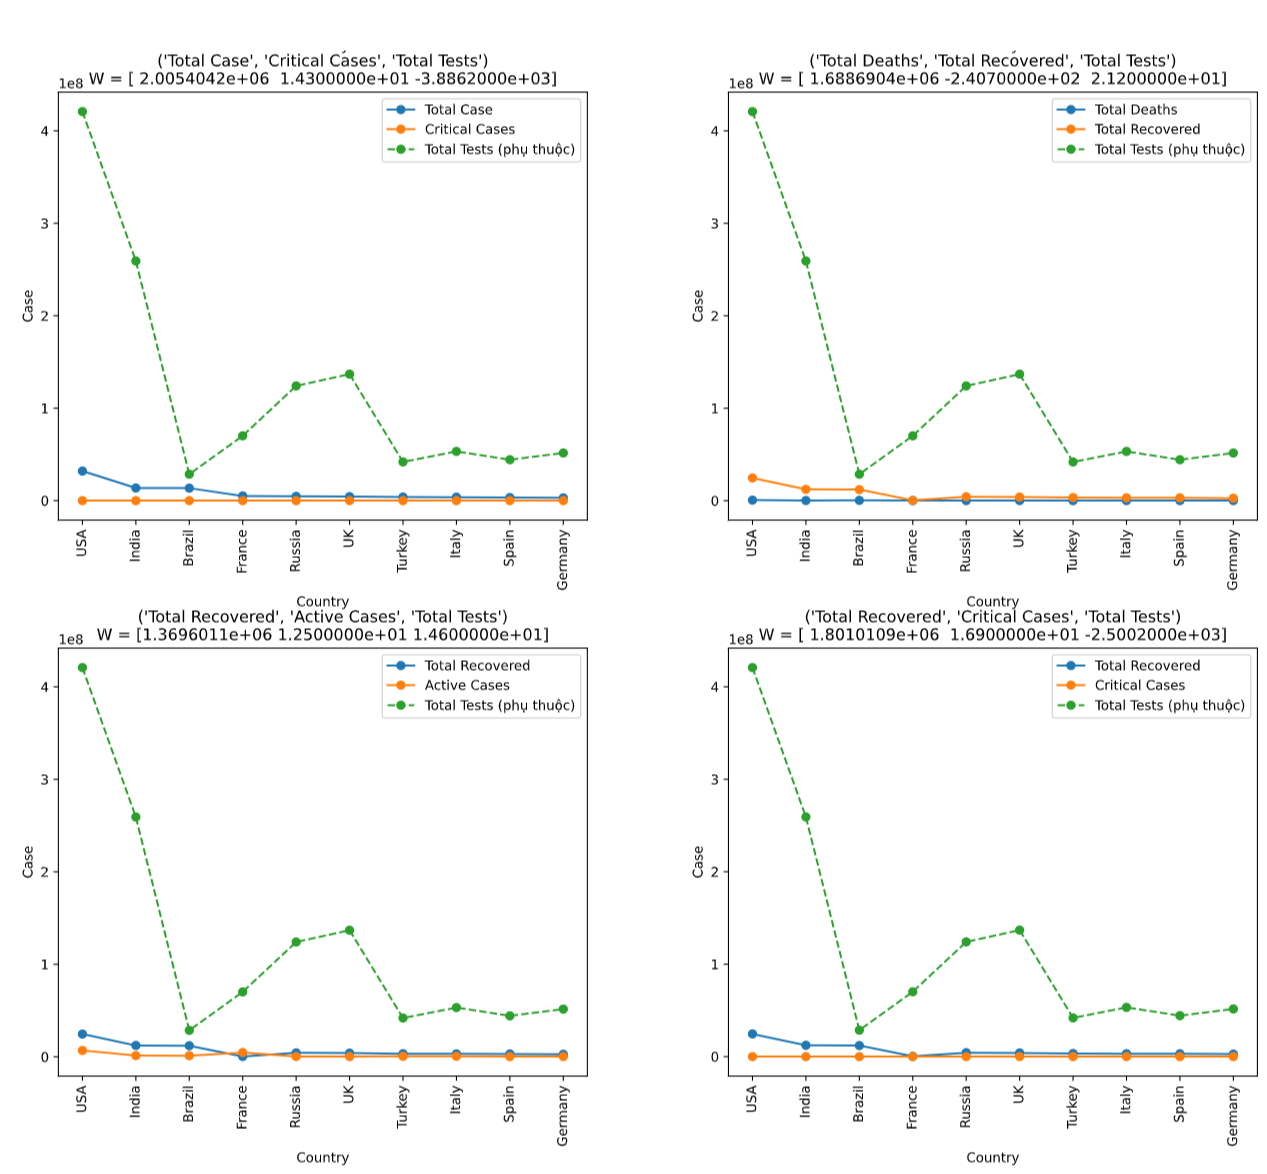
\includegraphics[scale=0.39]{img/relationship3Vars_1.png}
                \caption{Biểu đồ biểu diễn mỗi quan hệ giữa 3 biến dữ liệu}
            \end{center}
        \end{figure}

        \item Nhận xét dữ liệu: Từ Table 5, ta có thể kết luận rằng Var1 và Var2 có thể giải thích được từ 75\% đến 97\% sự thay đổi của Var3.
    \end{itemize}

    \subsection{Biểu diễn quan hệ giữa 4 trường dữ liệu}

    \begin{itemize}
        \item Tương tự như biểu diễn quan hệ giữa 3 biến dữ liệu, việc sử dụng biểu đồ đường cho biểu diễn quan hệ 4 biến cũng có thể trực quan được mỗi quan hệ này một cách rõ ràng với cơ sở toán học như đã trình bày ở phần \textit{4.3. Biểu diễn quan hệ giữa 3 trường dữ liệu}
        \item Các bộ 4 biến được xét tại đây thoả mãn điều kiện $R_{adj}^2 > 0.7$. Ta có bảng thống kê sau
        \begin{table}[H]
            \centering
            \begin{tabular}{|c|c|c|c|c|c|} 
            \hline
            \textbf{ STT } & \textbf{ Var1 (độc lập) } & \textbf{ Var2 (độc lập) } & \textbf{ Var3 (độc lập) } & \textbf{ Var4 (phụ thuộc) } & \textbf{ $R_{adj}^2$ }  \\ \hline
            1              & Total Case                & Total Deaths              & Total Recovered           & Active Cases                & 0.96                \\ \hline
            2              & Total Case                & Total Deaths              & Total Recovered           & Total Tests                 & 0.80                \\ \hline
            3              & Total Case                & Total Deaths              & Active Cases              & Total Tests                 & 0.80                \\ \hline
            4              & Total Case                & Total Deaths              & Critical Cases            & Total Tests                 & 0.80                \\ \hline
            5              & Total Case                & Total Recovered           & Active Cases              & Total Tests                 & 0.77                \\ \hline
            6              & Total Case                & Total Recovered           & Critical Cases            & Total Tests                 & 0.77                \\ \hline
            7              & Total Case                & Active Cases              & Critical Cases            & Total Tests                 & 0.77                \\ \hline
            8              & Total Deaths              & Total Recovered           & Active Cases              & Total Tests                 & 0.79                \\ \hline
            8              & Total Deaths              & Total Recovered           & Critical Cases            & Total Tests                 & 0.76                \\ \hline
            10             & Total Recovered           & Active Cases              & Critical Cases            & Total Tests                 & 0.77                \\\hline
            \end{tabular}
            \caption{Bảng các bộ 4 thuộc tính có mối tương quan trên 0.7}
        \end{table}

        \item Trực quan các bộ 4 biến
        \begin{figure}[H]
            \begin{center}
                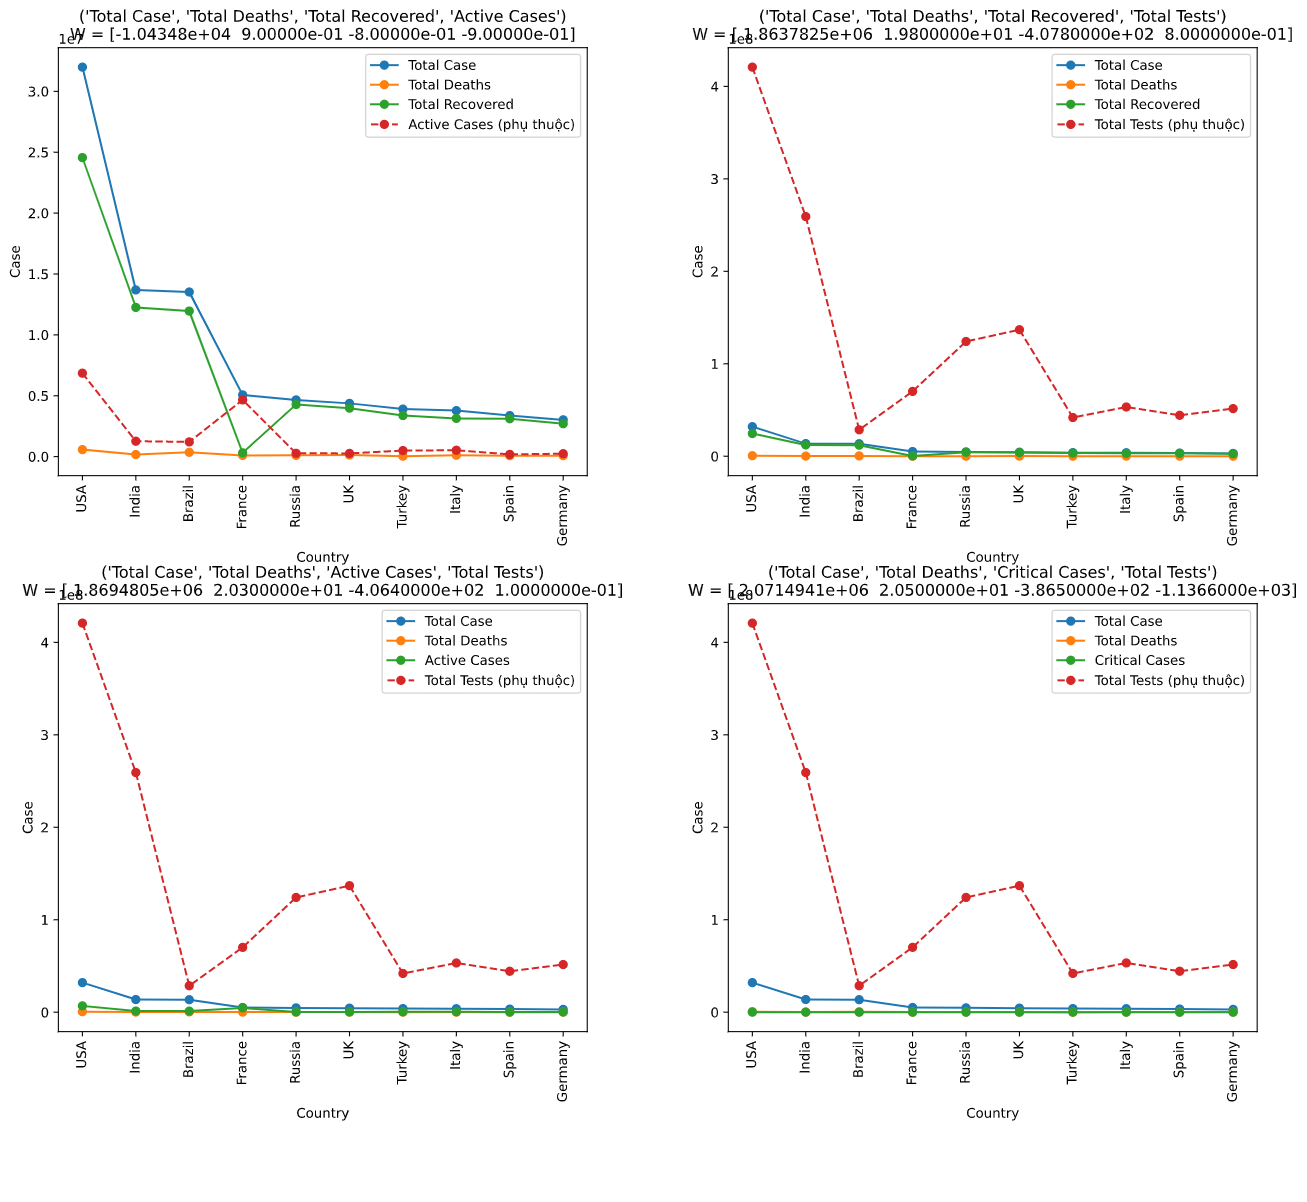
\includegraphics[scale=0.39]{img/relationship4Vars.png}
            \end{center}
        \end{figure}
        \begin{figure}[H]
            \begin{center}
                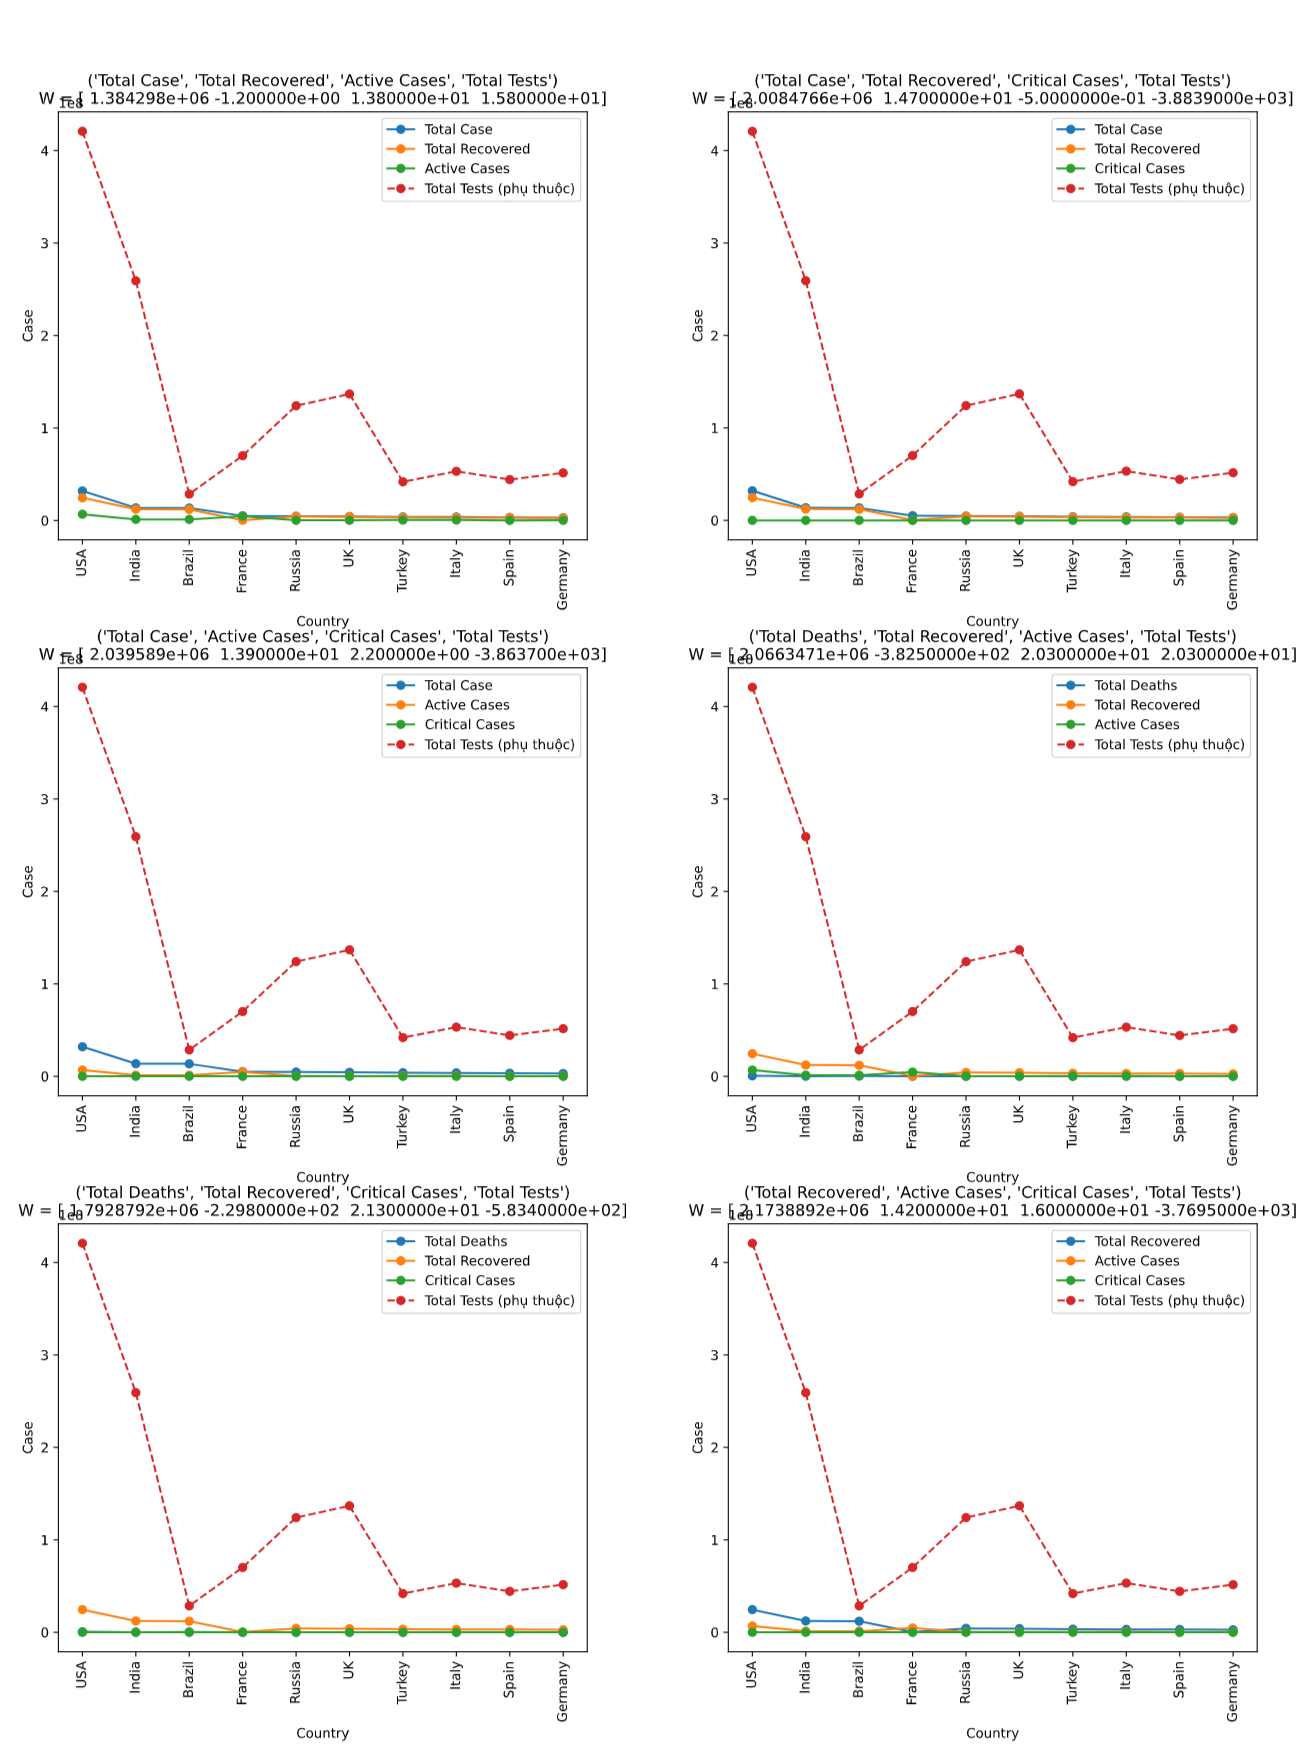
\includegraphics[scale=0.39]{img/relationship4Vars_1.png}
                \caption{Biểu đồ biểu diễn mỗi quan hệ giữa 4 biến dữ liệu}
            \end{center}
        \end{figure}

        \item Nhận xét dữ liệu: Từ Table 5, ta có thể kết luận rằng Var1, Var2 và Var3 có thể giải thích được từ 76\% đến 96\% sự thay đổi của Var4.
    \end{itemize}
    \clearpage

    \section{Một vài biểu diễn khác}

    \subsection{Stacked bar chart}

    \begin{itemize}
        \item Stacked bar chart dùng để biểu diễn một quan hệ 4 biến có sẵn (do \url{https://www.worldometers.info/} cung cấp)
        \begin{equation}
            Total cases = Total Deaths + Total Recovered + Active Cases
        \end{equation}

        \item Trực quan
        \begin{figure}[H]
            \begin{center}
                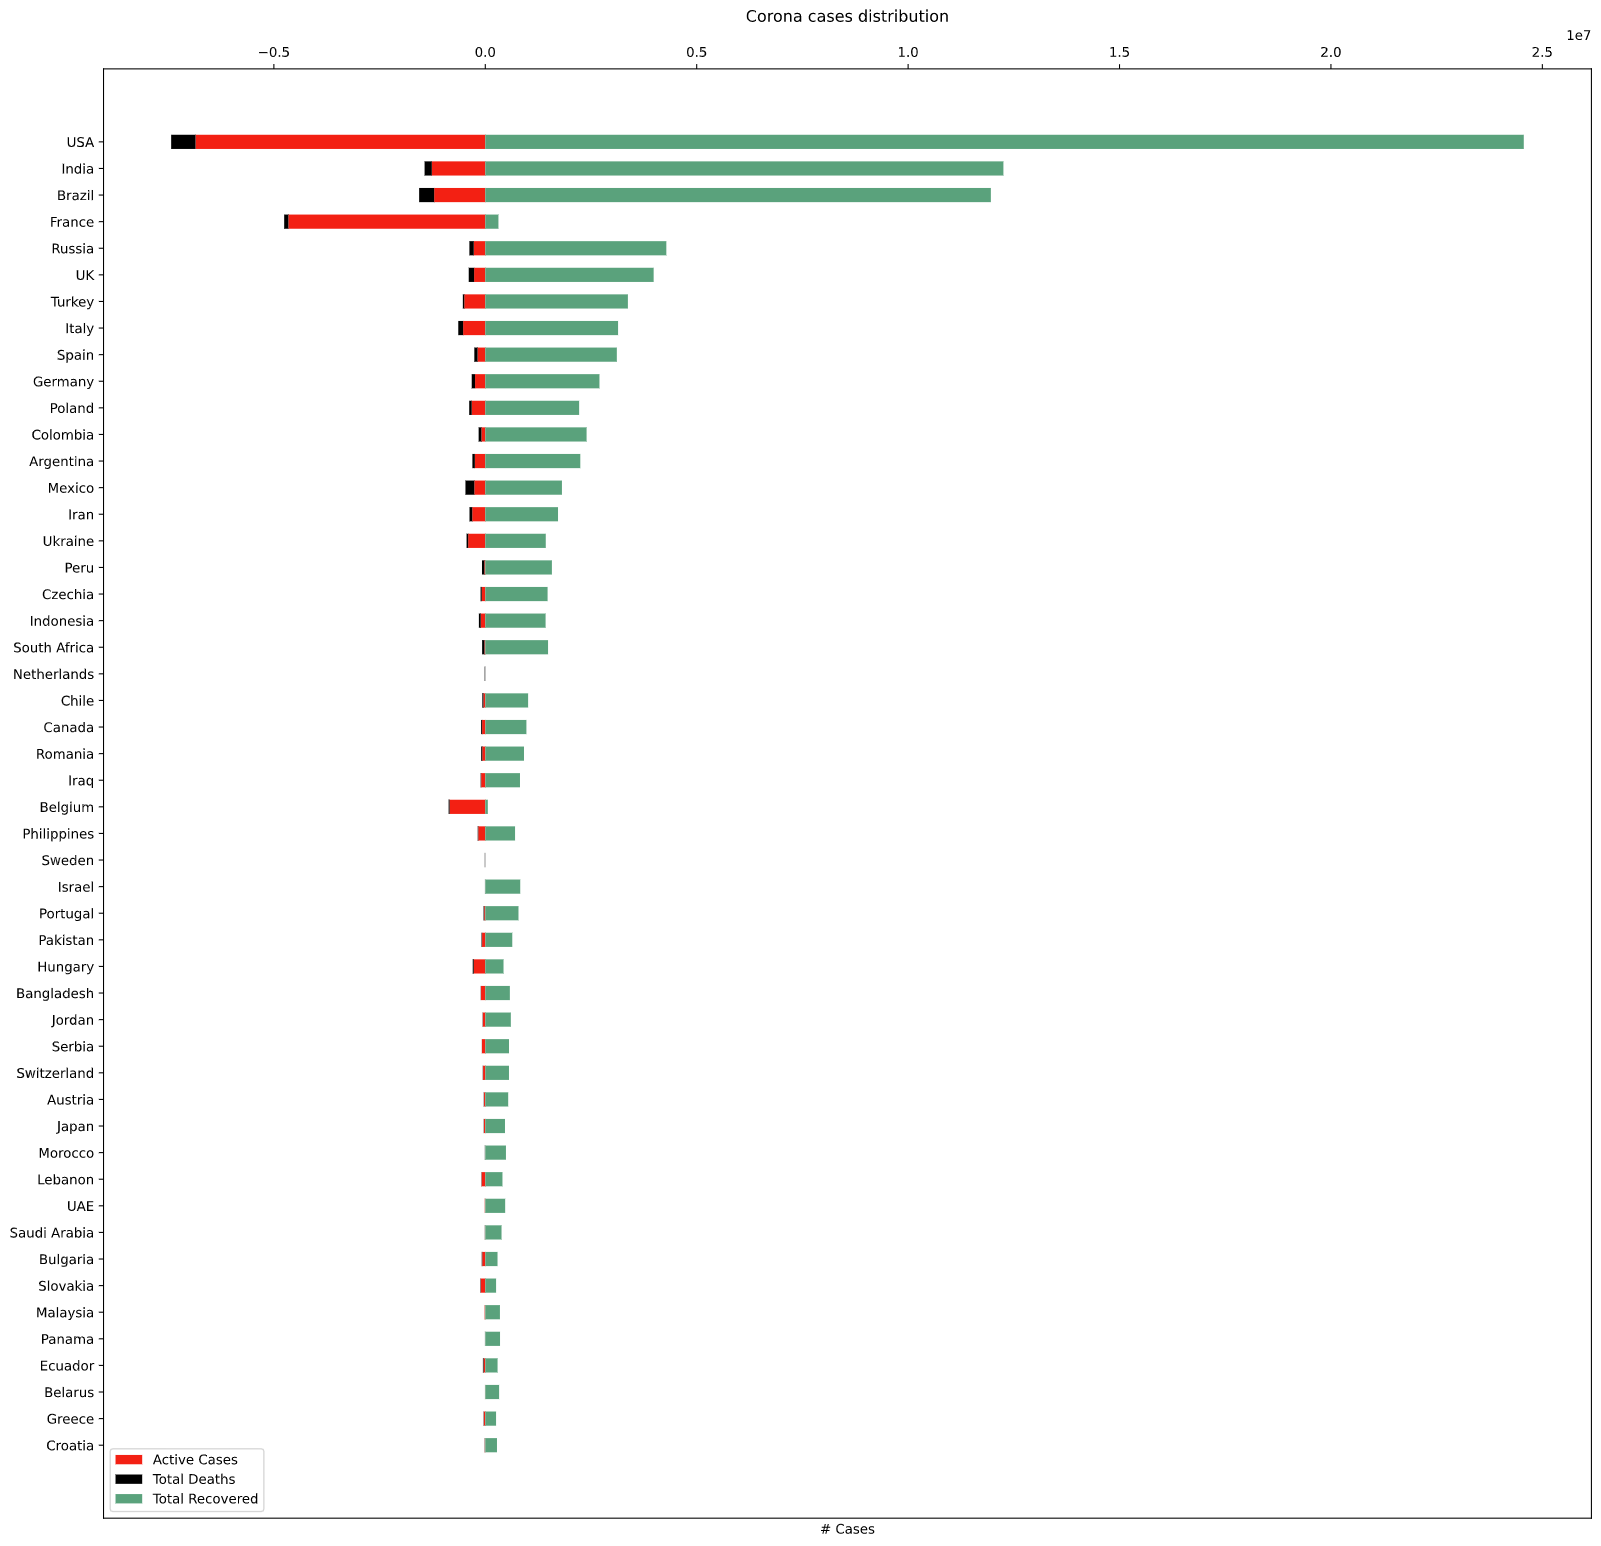
\includegraphics[scale=0.3]{img/stackedBar.png}
                \caption{Biểu đồ thể hiện quan hệ theo phương trình (4)}
            \end{center}
        \end{figure}

        \item Giải thích biểu đồ: Với mỗi nước được trực quan trên biểu đồ, chiều dài của cả cột chính bằng Total Cases của nước đó. Trong mỗi cột lại phân chia ra nhiều cột nhỏ như đã chú thích trong biểu đồ. Phần Total Deaths và Active Cases được vẽ hướng về phía âm - biểu thị số ca đã chết hoặc đang điều trị. Phần Total Recovered được tô màu xanh và hướng về phía dương - biểu thị số ca đã phục hồi. Ở đây, các nước được sắp xếp theo thứ tự giảm dần Total Cases.
        \item Lý do sử dụng stacked bar chart: Biểu đồ cột chồng rất có ích trong việc so sánh, xếp hạng dữ liệu tổng cũng như cho ta biết tỉ lệ của các thành phần tạo nên tổng. Trong trường hợp này, nó trực quan được rất rõ tỷ lệ hồi phục và tỷ lệ chết hoặc đang điều trị, thích hợp cho việc so sánh tổng số ca mắc giữa các quốc gia với nhau. 
    \end{itemize}

    \subsection{World map}

    \begin{itemize}
        \item Nếu việc trực quan bằng biểu đồ cột chồng là chưa đủ rõ ràng trong việc so sánh số liệu giữa các quốc gia cũng như đối chứng quan hệ giữa các biến dữ liệu thì biểu đồ world map như sắp trình bày dưới đây sẽ phần nào mang lại cảm giác trực quan rõ ràng hơn.
        \item Việc sử dụng world map cho ta thấy được cái nhìn tổng quan của mỗi biến dữ liệu giữa các quốc gia và thấy rõ được sự khác biệt giữa các quốc gia. Đồng thời cho ta dễ dàng thấy được những nét tương đồng giữa hai biến dữ liệu giữa các quốc gia, từ đó có thể nhận định được có sự tương quan xảy ra giữa hai biến dữ liệu đang xét không.
        \item Trực quan
        \begin{itemize}
            \item Tương quan giữa Total Cases với Total Deaths và Total Recovered
            \begin{figure}[H]
                \begin{subfigure}{.5\textwidth}
                    \centering
                    % include first image
                    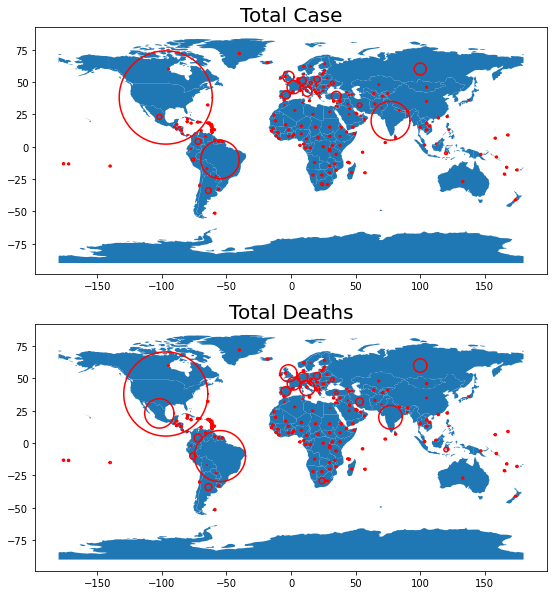
\includegraphics[width=1\linewidth]{img/case_death.png}  
                    \caption{Total cases - Total Deaths}
    
                \end{subfigure}
                \begin{subfigure}{.5\textwidth}
                    \centering
                    % include second image
                    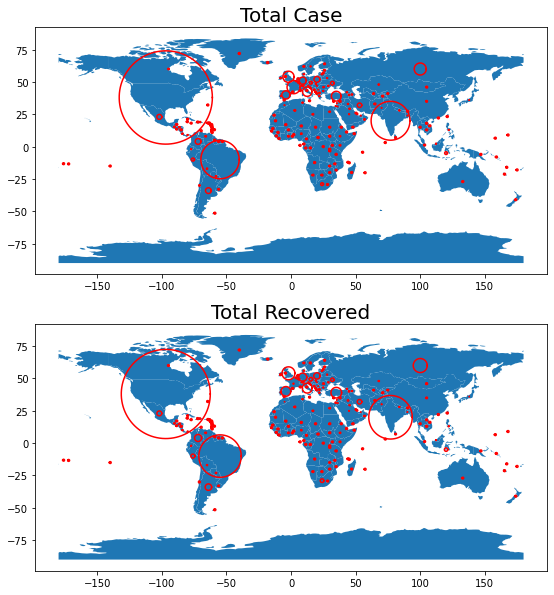
\includegraphics[width=1\linewidth]{img/case_recovered.png}  
                    \caption{Total cases - Total Recovered}
    
                \end{subfigure}
                \caption{Tương quan giữa Total Cases với Total Deaths và Total Recovered}
            \end{figure}

            \item Tương quan giữa Total Recovered với Total Deaths và Total Test
            \begin{figure}[H]
                \begin{subfigure}{.5\textwidth}
                    \centering
                    % include first image
                    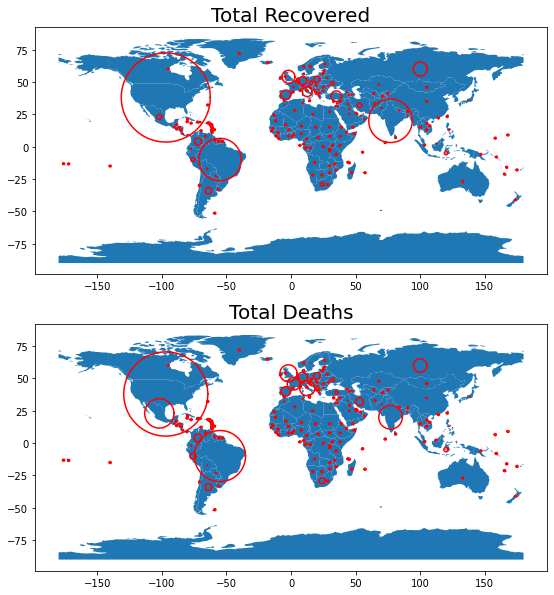
\includegraphics[width=1\linewidth]{img/recovered_death.png}  
                    \caption{Total Recovered - Total Deaths}
    
                \end{subfigure}
                \begin{subfigure}{.5\textwidth}
                    \centering
                    % include second image
                    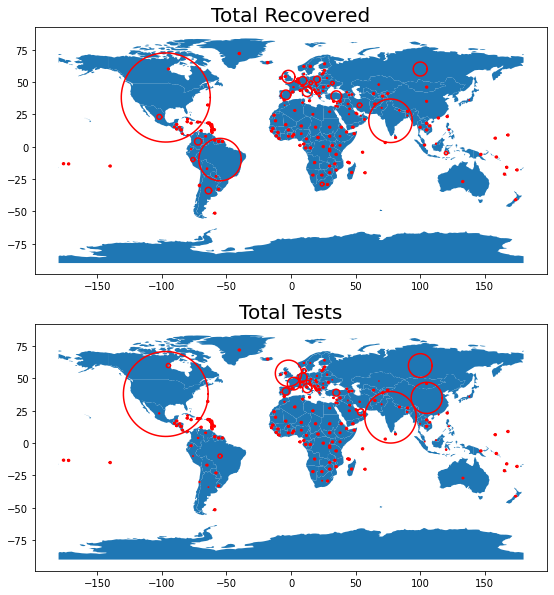
\includegraphics[width=1\linewidth]{img/recovered_test.png}  
                    \caption{Total Recovered - Total Test}
    
                \end{subfigure}
                \caption{Tương quan giữa Total Recovered với Total Deaths và Total Test}
            \end{figure}

            \item Tương quan giữa Total Cases với Total Test
            \begin{figure}[H]
                \begin{center}
                    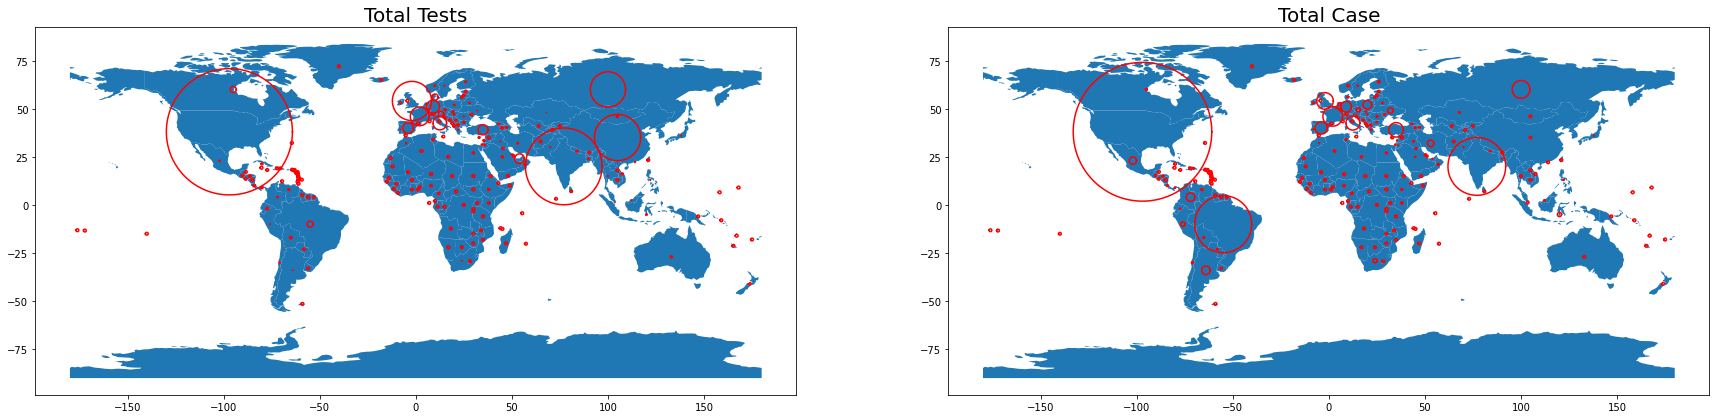
\includegraphics[scale=0.3]{img/test_case.png}
                    \caption{Tương quan giữa Total Cases với Total Test}
                \end{center}
            \end{figure}
        \end{itemize}
    \end{itemize}

    \clearpage

    \section{Tham khảo}

    \begin{enumerate}
        \item Các cơ sở toán học về thống kê và xấp xỉ tuyến tính được tham khảo trong cuốn "Thống kê máy tính tóm tắt" - TS. Bùi Tiến Lên
        \item Sử dụng framework Crawler: \url{https://gaire-crisna.medium.com/corona-data-scraping-with-scrapy-python-653a78340699}
    \end{enumerate}

    \clearpage

\end{document}
